%09/09 - Patricia Álvarez
\chapter{Introducción a la filogenia: principios y conceptos}
La filogenia es la determinación de la historia evolutiva de los organismos. Así, la filogenética es el estudio de: (i) la filogenia mediante el uso de árboles filogenéticos de los distintos organismos y (ii) las relaciones entre ellos. Ha habido varias iniciativas a lo largo de la historia (como \href{http://tolweb.org}{ToL Web}) que han intentado lograr crear árboles de todas las especies, cuyo número se estima por lo bajo que ronda los 3-5 millones. Estas estimaciones sobre la biodiversidad se realizan a partir de el número de grupos clave como los escarabajos, que son el grupo con mayor número de spp., en un lugar.

La filogenia es una disciplina muy consolidada; desde sus inicios, hace aproximadamente 200 años, sus representaciones no han cambiado mucho. La filogenia trabaja con árboles evolutivos, que son las \textbf{representaciones gráficas (patrones) de las relaciones ancestro-descendientes (relaciones históricas de parentescos) entre elementos}, que pueden ser especies, secuencias de genes, etc. Entender este patrón es esencial para realizar estudios comparativos de cualquier tipo, porque existen\textbf{ dependencias estadísticas entre los elementos que comparten ancestros comunes}. Conforme pasa el tiempo, se van aplicando diferentes y nuevos modelos evolutivos y se van depurando. En ultima instancia, se obtiene una mejor aproximación cuantos más datos se añadan (tanto más especies como más secuencias) a los modelos.

La filogenia sirve, entre otros, para: 
\begin{itemize}
\item Evolución de los seres vivos
\item Genómica: se puede observar mucho más allá y establecer límites entre especies. (Ej.: la evaluación es críptica. Si nos imaginamos a unos extraterrestres, no sabrán si clasificarnos a todos los humanos como una misma especie o distintas.)
\item Ingeniería genética
\item Farmacia
\item Epidemiología: ébola, VIH-1, etc. (Ver siguiente párrafo)
\item Biología de la conservación: discernir entre poblaciones y especies importa en relación con la clasificación de los espacios protegidos.
\item Control de plagas
\item Lingüística
\end{itemize}

La filogenética puede ser estudiada de diversas maneras. A menudo ha sido estudiada utilizando \textbf{registros fósiles}, que contienen información sobre la morfología de los antepasados de las especies actuales y la cronología de sus divergencias. Esto permite datar las filogenias. Sin embargo, el uso de registros fósiles presenta muchas limitaciones: pueden estar disponibles sólo para determinadas especies, los datos existentes de fósiles pueden estar fragmentados, la recolección de datos está limitada por la abundancia, hábitat, rango geográfico y otros factores; y las descripciones de los rasgos morfológicos son a menudo ambiguas (múltiples factores genéticos). Por todo esto, utilizar registros fósiles para determinar relaciones filogenéticas puede producir \textbf{sesgos}. Además, los fósiles de microorganismos son prácticamente inexistentes imposibilitando el uso de este enfoque. Afortunadamente, los \textbf{datos moleculares} que están en la forma de secuencias de ADN o de proteínas pueden ser también muy útiles para proporcionar una perspectiva de la evolución de los organismos, como el ARN 16S. Debido a que los genes son el medio para registrar las mutaciones acumuladas, éstos pueden servir como "fósiles moleculares". A través del análisis comparativo de secuencias de ADN de una serie de organismos relacionados, la historia evolutiva de los genes e incluso de los organismos puede ser revelada. La ventaja de utilización de datos moleculares es que son más numerosos que los registros fósiles y más fáciles de obtener. Además, no hay ningún sesgo de muestreo, como el que hay en los registros fósiles reales. Por tanto, es posible construir árboles filogenéticos más precisos y robustos utilizando datos moleculares. Como ejemplos, la filogenética se ha usado para datar y ubicar el origen del ébola en el brote de 2014 o el paciente 0 del VIH-1 en 1970.

Las filogenias, al ser una reconstrucción de la evolución de los caracteres, se construyen a partir de un registro/evidencias indirecto/as del proceso evolutivo. Por tanto, se deben realizar test de homología comprobar que los caracteres son comparables entre sí al compartir un origen común (homologías) y discernirlas de las homoplasias. De esa forma se obtiene información para construir clasificaciones y hacer predicciones dentro de un marco temporal cuando es posible obtenerlo.

\section{Conceptos básicos}
Los árboles filogenéticos suelen ser binarios, estando compuestos por \textbf{nodos externos o terminales} y \textbf{nodos internos} unidos por \textbf{ramas} que parten de una \textbf{raíz}. A través de las diferentes ramas se van reconstruyendo las relaciones entre las especies. Los \textbf{nodos internos son hipótesis evolutivas de posibles ancestros comunes} de los cuales normalmente faltan datos para confirmar o descartar la teoría. En las distintas ramas se pueden representar la transformación de caracteres que aparecen a nivel genético y que se transmiten por herencia.  

\begin{figure}[htbp]
\centering
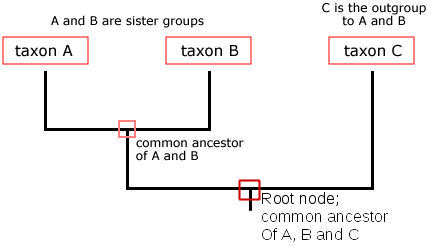
\includegraphics[width=0.5\linewidth]{figs/taxon-tree.png}
\caption{Partes de un árbol filogenético.}
\end{figure}

Se denominan \textbf{grupos hermanos} a los nodos terminales que parten de un mismo nodo interno, es decir, dos taxones que compartan un ancestro común no compartido por ningún otro taxón. El \textbf{grupo externo (outgroup)} es aquel que se encuentra más alejado y parte de una rama distinta desde la raíz. Normalmente, este outgroup se elige arbitrariamente para poder colocar la raíz donde se estima correcto. Todas las especies que se desarrollan desde una rama de la raíz se denomina \textbf{grupo interno o ingroup}. 

Los árboles filogenéticos se pueden representar sin enraizar o enraizado. Un árbol filogenético sin raíz no asume conocimiento de un ancestro común, solo posiciones de los taxones para mostrar sus relaciones relativas (no hay dirección de un camino evolutivo). Para describir la dirección de la evolución se necesita un árbol filogenético con raíz donde todas las secuencias bajo estudio tienen un ancestro o nodo raíz común (más informativo). Mientras que los árboles filogenéticos se centran en las relaciones evolutivas entre diferentes especies, las redes haplotípicas son representaciones gráficas sobre las relaciones evolutivas entre las diferentes poblaciones.

A la hora de visualización, hay varias formas de representar los árboles filogenéticos. Los distintos elementos no tienen un orden concreto; da igual si en un árbol los nodos terminales están en distinto orden mientras que las ramas sigan el mismo camino. En general, se suelen poner los nodos terminales de manera que sea más fácil de leer a simple vista.

\begin{figure}[htbp]
\centering
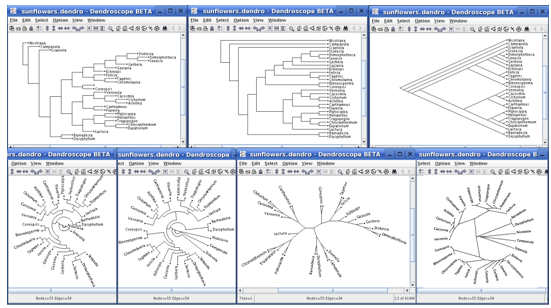
\includegraphics[width=0.5\linewidth]{figs/representaciones-arboles.png}
\caption{Distintas representaciones de los árboles filogenéticos.}
\end{figure}

\section{Politomías}
La topología es la forma en que se ramifica un árbol. Cuando todas las ramas se bifurcan en un árbol filogenético, éstas son denominadas como una \textbf{dicotomía}. Por el contrario, si de un nodo surgen más de dos ramas (descendientes), entonces se denomina \textbf{politomía}.

\begin{figure}[htbp]
\centering
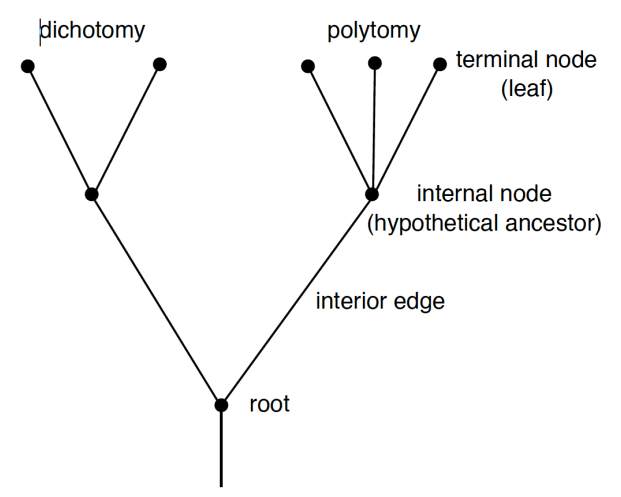
\includegraphics[width=0.3\linewidth]{figs/dichotomy-polytomy.png}
\caption{Diferencia entre dicotomía y politomía.}
\end{figure}

Los árboles filogenéticos se consideran resueltos cuando de un nodo interno salen las distintas terminales. En la mayoría de casos, los árboles son no resueltos y tienen politomías, es decir, que desde un nodo interno no se sabe cómo han avanzado las especies. A partir de ahí solo se pueden añadir más datos, pintar uniones con un bootstrap bajo (es decir, un bajo soporte de esa bifurcación), o justificar que estamos atestiguando un momento de especiación. Dentro de las hipótesis filogenéticas siempre hay más de una solución (se producen varios árboles igualmente óptimos), así que el árbol final se debe elegir. Un árbol de consenso puede ser construido mostrando las porciones de bifurcación resueltas comúnmente y colapsando aquellas que no concuerdan entre los árboles. En un árbol de consenso estricto, todos los nodos en conflicto son colapsados.

\begin{figure}[htbp]
\centering
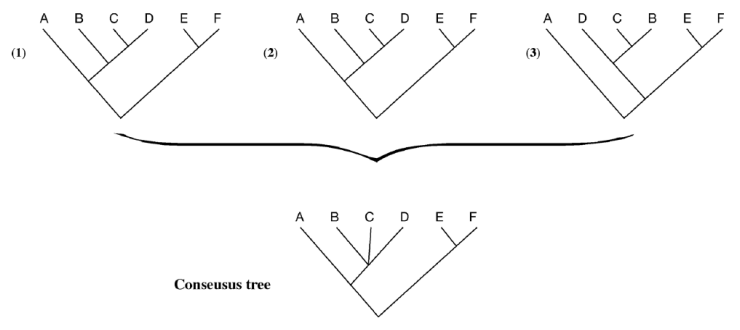
\includegraphics[width=0.5\linewidth]{figs/consensus-tree.png}
\caption{Árbol de consenso.}
\end{figure}

\section{Tipos de árboles filogenéticos}
Existen distintos tipos de árboles filogenéticos. Los \textbf{filogramas (phylogram}) miden en las ramas los cambios que ha habido por sitio, por lo que las longitudes de las ramas representan a escala la cantidad de divergencia evolutiva. Tienen la ventaja de mostrar tanto las relaciones evolutivas como la información sobre el tiempo relativo de divergencia de las ramas. Los \textbf{cladogramas (cladogram)} muestran la similitud de los distintos elementos, pero las longitudes de sus ramas no son proporcionales al número de cambios evolutivos y, por tanto, no tienen ningún significado filogenético. Los \textbf{cronogramas (chronogram)} representan la relación de los elementos de forma temporal.

\begin{table}[h]
\centering
\begin{tabular}{l c c}
\hline
\multicolumn{1}{l}{[phyl(o) gr. 'raza', 'estirpe']} & \multirow{3}{1em}{+} & \multirow{3}{12em}{[-gram-ma gr. 'representación gráfica']} \\
\multicolumn{1}{l}{[klad(o) gr. 'rama']} & & \\
\multicolumn{1}{l}{[khron(o) gr. 'tiempo']} & & \\
\hline
\end{tabular}
\caption{Tabla con términos griegos y sus significados.}
\end{table}

\begin{figure}[htbp]
\centering
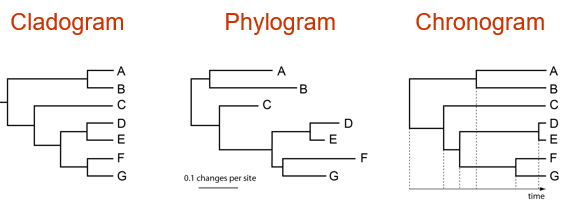
\includegraphics[width=0.5\linewidth]{figs/tipos-arboles.png}
\caption{Tipos de árboles filogenéticos.}
\end{figure}

\section{Inferencia filogenética}
Cualquier episodio histórico es, por definición, irrecuperable. La única forma que tenemos de reconstruirlo es a través del estudio de sus efectos. Por ello, la reconstrucción filogenética es un proceso de inferencia: se intenta obtener la mejor estimación posible de una historia evolutiva basada en la información incompleta y con frecuencia ruidosa contenida en los datos. Las evidencias que se emplean se basan en la morfología (comparación entre caracteres de especies), la ultraestructura (cortes vistos al microscopio electrónico), embriología (fases del desarrollo embrionario), la paleontología (registro fósil), la etología (comportamiento animal para estudiar evolución simpátrica), la bioquímica y las moléculas. 

Un \textbf{carácter} es una característica de los taxones que, en principio, es heredada (si no es heredada, no se puede utilizar la filogenia). El \textbf{estado de carácter} es el valor específico que toma un carácter en un taxón concreto. Por ejemplo, un carácter sería tener ojos y el estado de ese carácter sería 2 para humanos y 8 para algunas arañas.

\section{Homología}
La \textbf{homología} es la relación que existe entre dos partes orgánicas diferentes de dos organismos distintos cuando sus determinantes genéticos tienen el mismo origen evolutivo, es decir, cuando un mismo órgano tiene diversas formas y funciones. Los caracteres que se estudian en filogenia deben ser homólogos. Se compara la semejanza de una estructura debido a la herencia común. Por el contrario, la analogía es una estructura semejante a otra o que tiene la misma función, pero cuyo desarrollo embrionario y origen son diferentes. No se presentan en un antepasado común (como en el caso de los caracteres homólogos), si no que es fruto de convergencia evolutiva.

En genética y biología molecular, también existe homología en las secuencias. Se distinguen dos tipos: la ortología y la paralogía. Los \textbf{genes ortólogos} son semejantes por pertenecer a dos especies que tienen un antepasado común. Los \textbf{genes parálogos} son aquellos que se encuentran en el mismo organismo y cuya semejanza revela que uno procede de la duplicación del otro (y puede adquirir funciones diferentes del gen original). La ortología requiere que se haya producido especiación, mientras que esta no es necesaria en el caso de la paralogía, que puede producirse solo en los individuos de una misma especie. Por ello, idealmente se deben comparar caracteres ortólogos para hacer las reconstrucciones filogenéticas.

\begin{figure}[htbp]
\centering
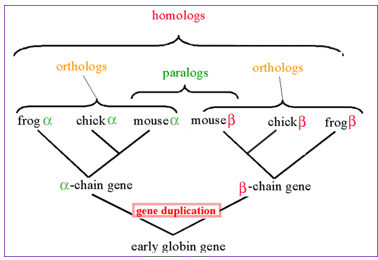
\includegraphics[width=0.5\linewidth]{figs/ortologos-paralogos.png}
\caption{Homología en genes de la hemoglobina.}
\end{figure}

%11/09 - Patricia Álvarez
\subsection{Tipos de homología}
En cladística, se emplean unas clasificaciones de las propiedades de organismos basándose en similitudes derivadas. Una \textbf{plesiomorfía} se refiere al estado \textit{ancestral} (o \textit{primitivo}) de un carácter que comparten distintas especies por heredarlo del antepasado común; en el árbol filogenético de ejemplo se presenta en los ancestros y los grupos externos. En contraposición, la \textbf{apomorfía} es un carácter novedoso evolutivamente y se dice que es \textit{derivado}, ya que deriva de otro rasgo perteneciente a un taxón ancestral filogenéticamente próximo. Así, se emplean los adjetivos plesiomófico y apomórfico en lugar de primitivo y avanzado para evitar juicios de valor sobre la evolución de los carácteres. 
Además, una \textbf{sinapomorfía} es una apomorfía (carácter exclusivo) compartida por un ancestro común y todos sus descendientes; y una \textbf{simplesiomorfía} se refiere a una plesiomorfía (carácter ancestral) compartida por dos o más taxa. Finalmente, una \textbf{autapomorfía} es un carácter novedoso y único de un taxón que no aparece en el antepasado, por lo que no lo comparte con ningún otro. 

\begin{table}[htbp]
\begin{mdframed}[backgroundcolor=black!10]
    \centering
    El prefijo "sin" viene de "compartido". Por tanto, los caracteres sinapomorfos son caracteres apomorfos compartidos, mientras que las simplesiomorfías son plesiomorfías compartidas.
    \end{mdframed}
\end{table}

\begin{table}[h]
\centering
\begin{tabular}{l c c }
\hline
\multicolumn{1}{l}{[sýn- gr. 'con', 'unión']} & \multirow{4}{*}{+} & \multirow{2}{*}{[morph gr. 'forma']} \\
\multicolumn{1}{l}{[plēsio- gr. 'cercano']} & &  \\
\multicolumn{1}{l}{[aut(o)- gr. 'que actúa por sí mismo']} & & \multirow{2}{*}{[-íā gr. 'cualidad']}  \\
\multicolumn{1}{l}{[apó- gr. 'a partir de' (derivado, novedoso)]} & & \\
\hline
\end{tabular}
\caption{Tabla con términos griegos y sus significados.}
\end{table}

\begin{figure}[htbp]
\centering
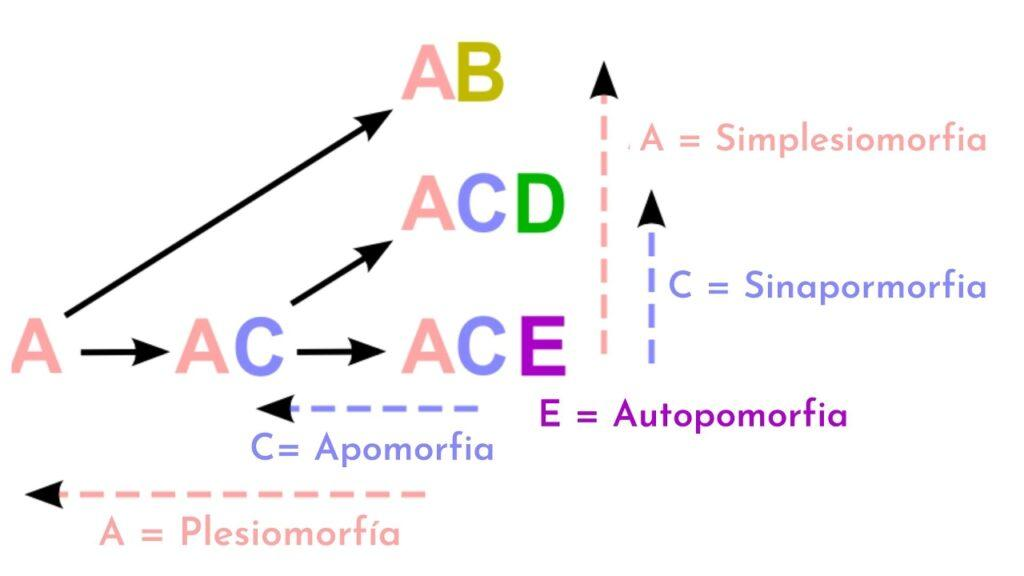
\includegraphics[width=0.5\linewidth]{figs/sinapomorfia.jpg}
\caption{Tipos de homología en el árbol filogenético (tumbado). El carácter A es plesiomórfico al estar en el ancestro. El carácter C es apomórfico al ser una novedad evolutiva. En los nodos terminales, el carácter A se considera simplesiomórfico al estar compartido por los descendientes y ser un carácter ancestral. Por el contrario, el carácter C en los nodos terminales es sinapomórfico por ser un carácter novedoso y estar compartido en el ancestro en el que surgió y sus descendientes. Los caracteres B, D y E son autopomorfos por estar presentes en un único nodo terminal.}
\end{figure}

\subsection{Homoplasia}
La homoplasia es el cambio evolutivo paralelo que hace que dos organismos presenten un mismo carácter adquirido independientemente. La \textbf{convergencia} se da cuando dos estructuras similares han evolucionado independientemente a partir de estructuras ancestrales distintas y por procesos de desarrollo diferentes. Se considera que el \textbf{paralelismo} involucra patrones de desarrollo similares en líneas evolutivas diferentes, pero próximas. La diferencia con la convergencia es que en el paralelismo, hay un ancestro que no presenta un carácter y dos descendientes directos sí presentan esa novedad evolutiva, mientras que en la convergencia los descendientes con carácter no tienen el mismo ancestro común directo. No obstante, en la práctica, la distinción entre convergencia y paralelismo es un tanto arbitraria porque no existe una regla exacta para limitar la antigüedad del antepasado común. Finalmente, en la \textbf{reversión}, un organismo adquiere un carácter de sus antepasados más lejanos. Esto implica que uno o más caracteres adquiridos previamente se han eliminado y se han vuelto a los más anteriores. 

\begin{figure}[htbp]
\centering
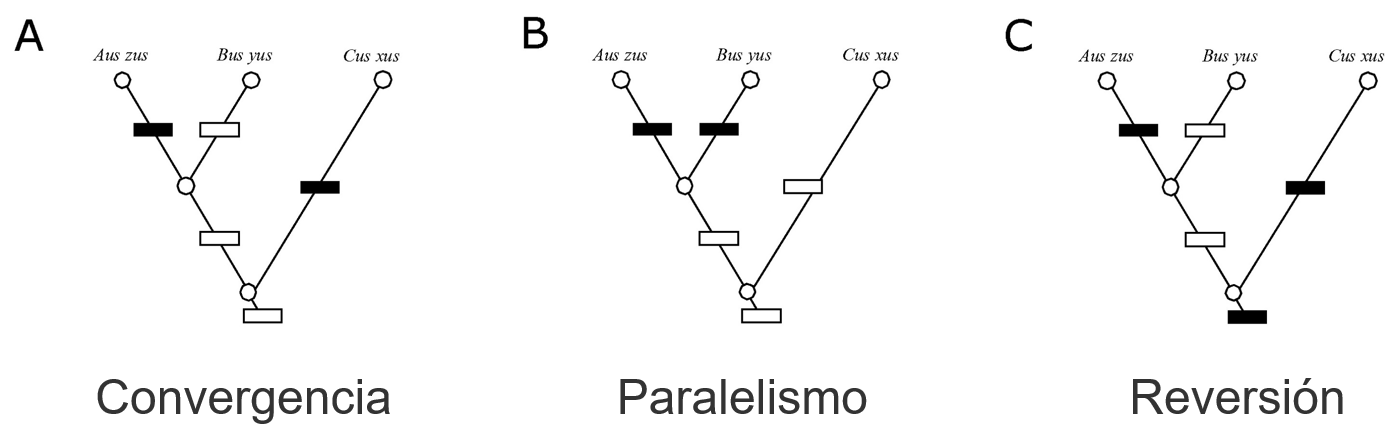
\includegraphics[width=0.5\linewidth]{figs/homoplasia.png}
\caption{Diferencias entre convergencia, paralelismo y reversión.}
\end{figure}

\subsection{Agrupamientos}
Un \textbf{grupo monofilético} es un clado que contiene un ancestro y todos sus descendientes, formando así un solo grupo evolutivo. Un \textbf{grupo parafilético} es similar, pero excluye a algunos de los descendientes que han sufrido cambios significativos. Un grupo con miembros de líneas evolutivas separadas se llama \textbf{polifilético}, conteniendo así grupos de especies con distintos ancestros comunes. 

\begin{figure}[htbp]
\centering
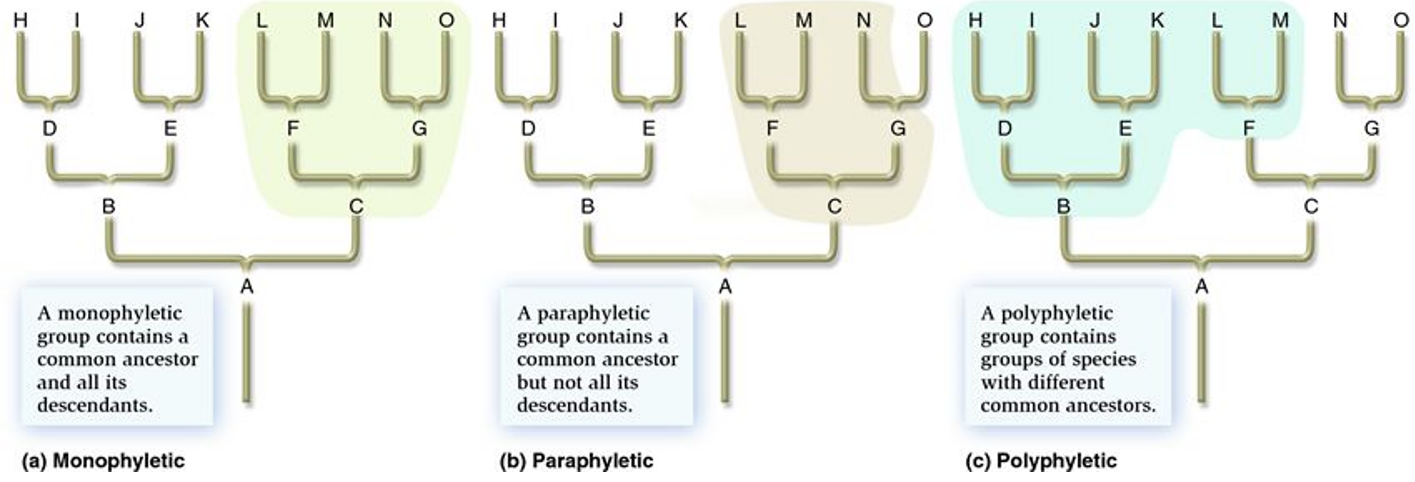
\includegraphics[width=0.5\linewidth]{figs/agrupamientos.png}
\caption{Agrupamientos de grupos monofiléticos, parafiléticos y polifiléticos.}
\end{figure}

De esa forma, los grupos monofiléticos presentan sinapomorfía, los grupos parafiléticos presentan simplesiomorfía, y los grupos polifiléticos homoplasia. 

\begin{figure}[htbp]
\centering
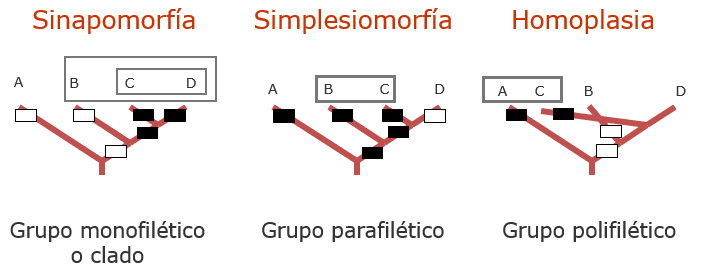
\includegraphics[width=0.5\linewidth]{figs/homoplasia-agrupamientos.png}
\caption{Grupos y caracteres que se apoyan.}
\end{figure}

\subsection{Fenotipo vs moléculas}
Tradicionalmente se han empleado los \textbf{carácteres fenotípicos} para establecer las relaciones filogenéticas. Esto se debe a que suelen ser carácteres evolutivamente relevantes y complejos menos proclives a la homoplasia. Además, son los únicos carácteres disponibles en algunos casos como en fósiles o especímenes raros. No obstante, puede haber problemas de codificación de taxones supraespecíficos como terminales (quimera) y se pueden dar casos de subjetividad en la codificación de carácteres. Además, hay un número limitado de carácteres fenotípicos y podemos encontrar taxones altamente autapomórficos. 

Recientemente se están empleando \textbf{carácteres moleculares} al ser estrictamente heredables y no haber ambigüedades en la codificación. Por ello, determinar el estado de los carácteres es trivial. Hay ciertas regularidades en la evolución de los carácteres moleculares, y éstos son robustos frente a la distancia evolutiva. También son muy abundantes y ofrecen información temporal. El problema de los carácteres moleculares es que son más proclives a la homoplasia al tener solo 4 nucleótidos y 20 aminoácidos. La evolución de estos carácteres es compleja. Además, los árboles de genes no siempre coinciden con los árboles de especies. La determinación de la homología puede ser difícil por duplicación o pérdida de genes y alineamientos. 

Se suelen utilizar multitud de genes separados y analizarlos de forma separada. El consenso de análisis separados es una estimación conservadora de la filogenia. Algunos métodos filogenéticos sólo se pueden aplicar a ciertos tipos de datos. A nivel de especies, la concatenación de genes diferentes puede ser inapropiada si se da transferencia horizontal de genes, hibridación, duplicación de genes o coalescencia más profunda que el tiempo de divergencia. El conflicto entre caracteres se resuelve teniendo en cuenta toda la evidencia disponible y realizando análisis combinados. Diferentes tipos de datos proporcionan información a diferentes niveles filogenéticos. La señal filogenética aumenta debido a la congruencia entre caracteres de diferentes conjuntos de datos. 

Es importante que el conjunto de datos sea lo más completo posible. Es necesario hacer un muestreo de taxones (incluyendo los grupos externos) y genes razonable y justificado. 
